\section{Diagrammes}
\label{sec:diagrammes}

Afin de gérer le projet, j'ai utilisé plusieurs logiciels. \\

Pour la création du diagramme de \textbf{Gantt}, j'ai d'abord employé \textit{GanttProject} qui ne m'a pas permis d'avoir deux tâches décallées en parallèle. Je me suis alors tourné vers \textit{Microsoft Project} qui, lui, m'a donné satisfaction. \\

Quant à celui de \textbf{PERT}, je l'ai conçu \textit{à la main}, car aucun outil ne proposait de concevoir le diagramme selon les instructions données dans le cours.

\newpage


\subsection{Gantt}
\label{subsec:gantt}

Voici le diagramme de Gantt du projet et son tableau descriptif :

%\vspace{0.5cm}

\begin{figure}[!h]
    \centering
    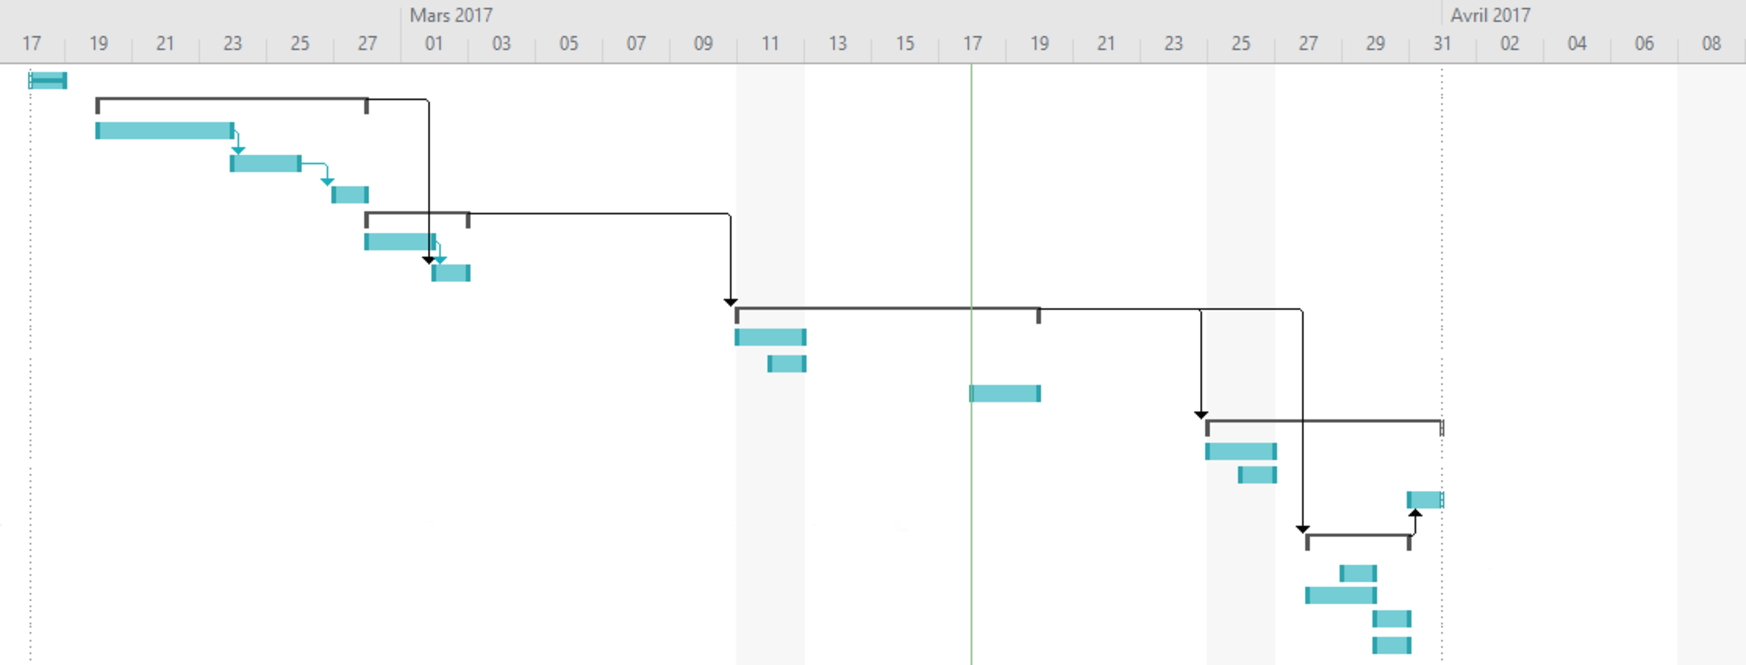
\includegraphics[scale=0.5]{textures/images/diagrammes/DiagrammeDeGantt.pdf}
    \caption{Diagramme de Gantt}
\end{figure}
\begin{figure}[!h]
    \centering
    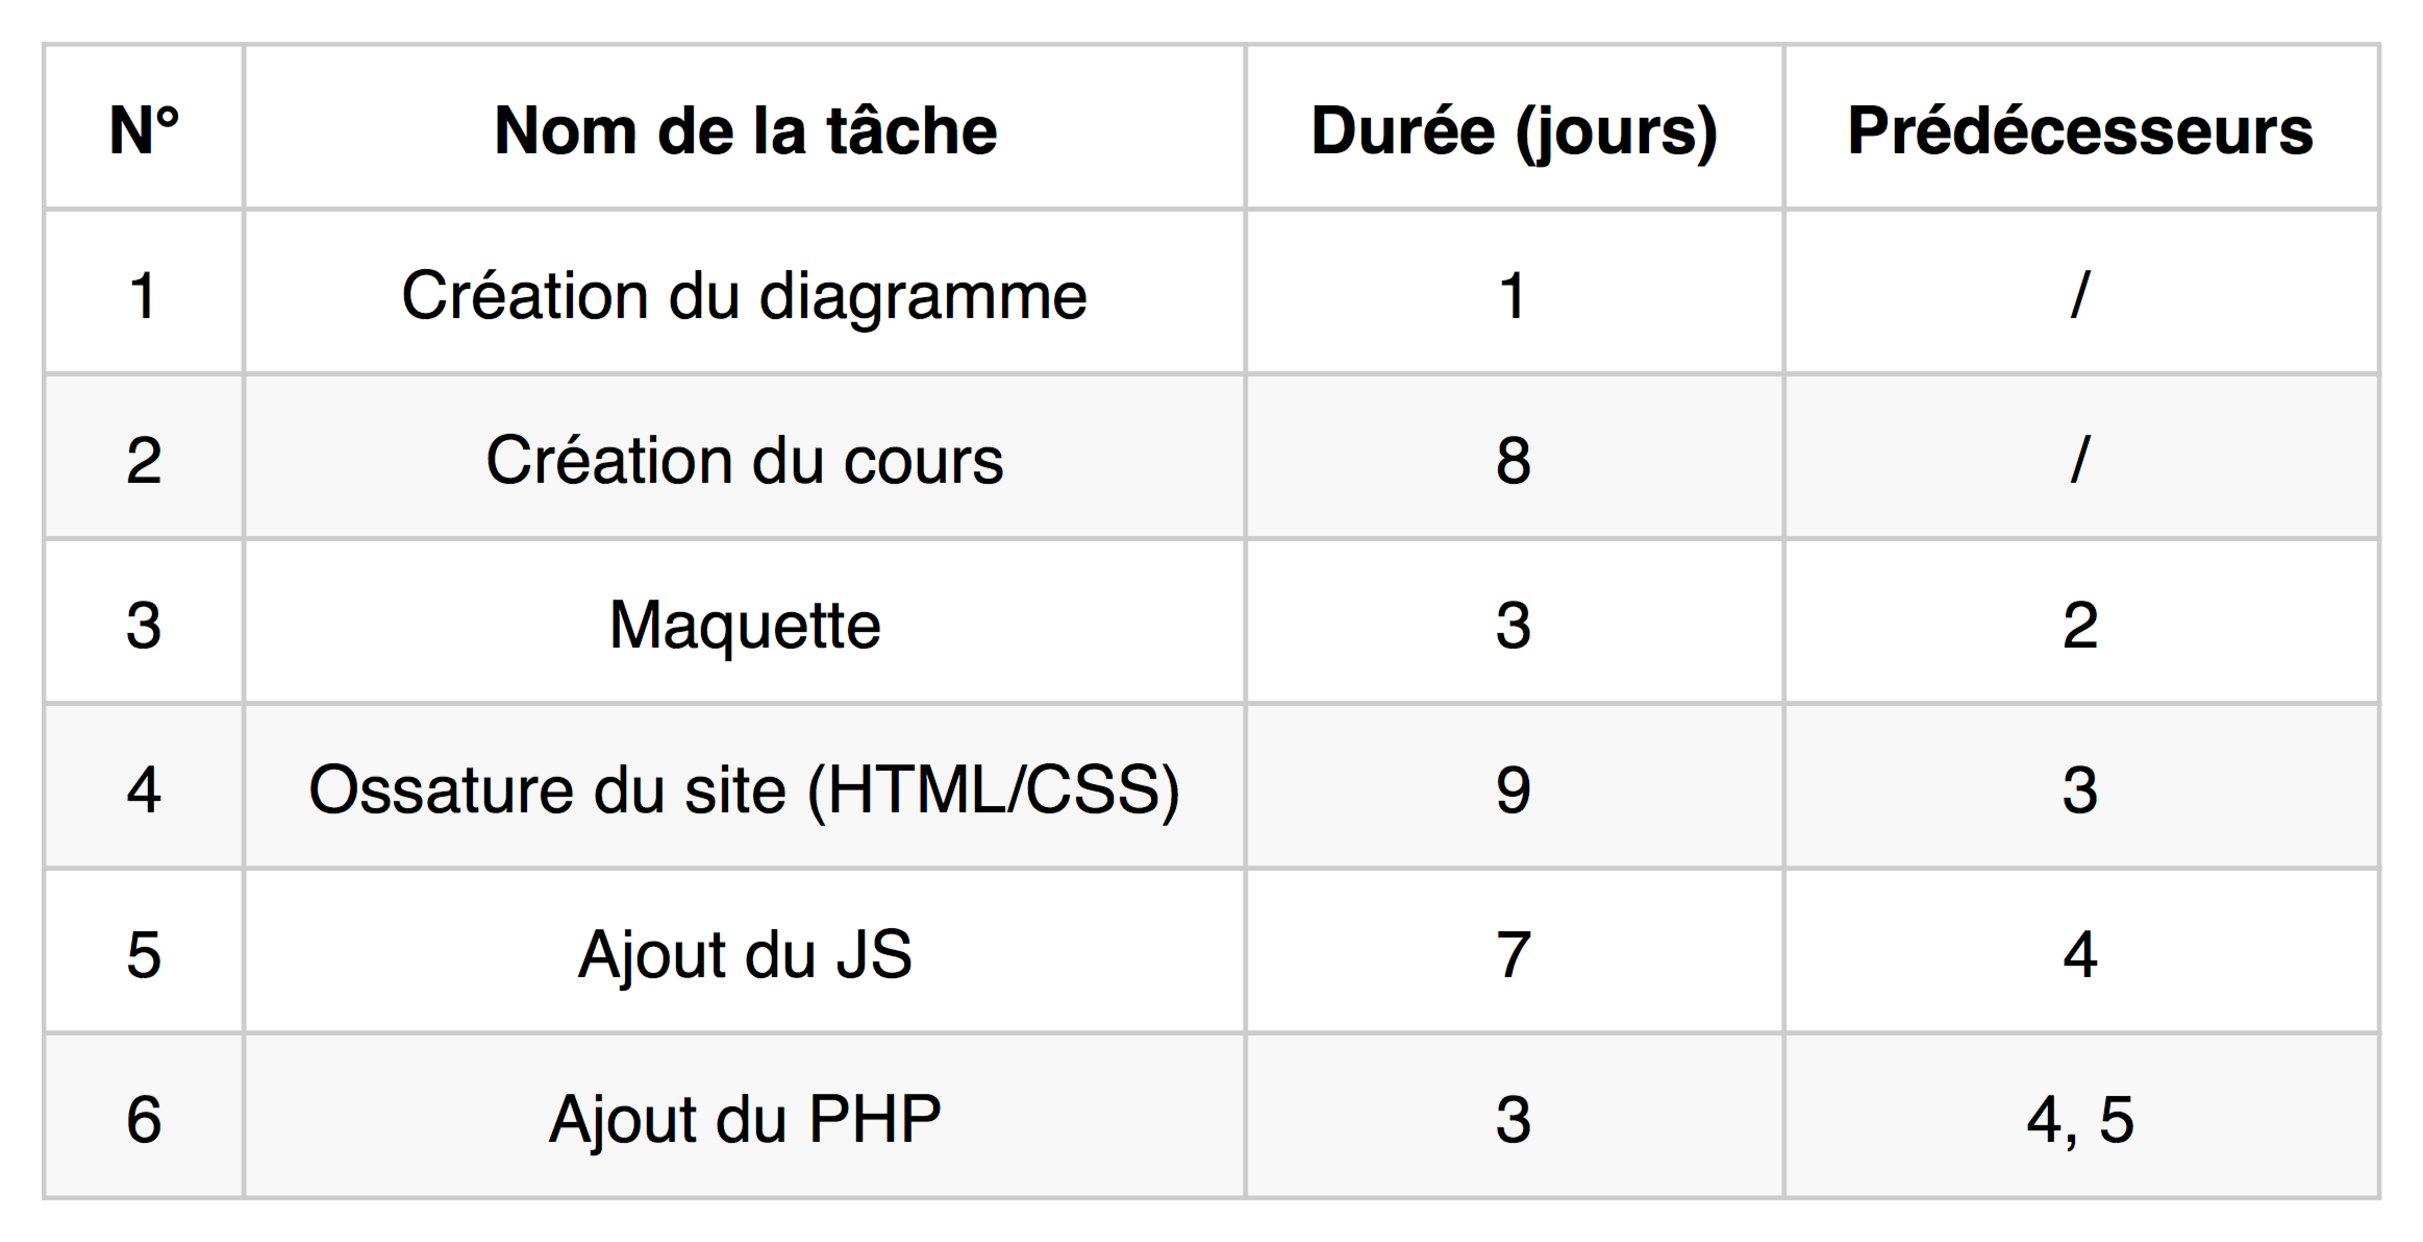
\includegraphics[scale=0.3]{textures/images/diagrammes/TableauDeGantt_brief.pdf}
    \caption{Tableau descriptif}
\end{figure}

Comme on peut le voir, la durée totale prévue du projet est de 31 jours.\\

Le projet est découpé en 6 tâches principales détaillées ci-dessous. \\

La création du diagramme a duré moins d'un jour, mais c'était la durée minimale disponible dans \textit{Microsoft Project}… \\

\newpage

La création du cours comprend l'écriture des différents chapitres et questionnaires. \\
Comme dit précédemment, celle-ci s'est déroulée en deux étapes :
\begin{enumerate}

    \item L'écriture d'un premier jet de trois chapitres : les variables, les booléens et la complexité, et… de quelques exercices.
    \item La réécriture des chapitres sur les variables et les booléens, et l'écriture des autres chapitres \textit{(l'introduction, les conditions et les boucles)}. Chacun accompagné de son questionnaire principal et de ses questionnaires secondaires. \\
    Le questionnaire principal teste, en quatre questions, les connaissances acquises tout au long du chapitre, tandis que les secondaires testent celles de la page précédente en deux questions.\\
    
\end{enumerate}

Cinq maquettes ont été créées :
\begin{enumerate}

    \item La page d'accueil, très \textit{(trop)} simple et sobre;
    \item La page du cours comprenant les liens vers les chapitres;
    \item L'aperçu d'un chapitre. C'est la raison pour laquelle les maquettes dépendent de la tâche précédente;
    \item La page des trophées;
    \item La page du compte de l'utilisateur. \\
    
\end{enumerate}

Dans la version finale, on peut remarquer que le design a évolué. Comme lors d'une démonstration, celui-ci a été jugé \og \textit{trop simple} \fg j'en ai profité pour ajouter des \textbf{animations} sur la page d’accueil, sur les chapitres ainsi que sur les trophées, et de la \textbf{coloration syntaxique} du code. \\

La création de l'ossature du site fut la partie la plus longue parce que la majorité du code du site a été écrite à ce moment. \\
Ainsi, toutes les pages \textit{(accueil, cours, chapitres, trophées, etc.)}, styles et effets CSS ont été créés et n'ont plus été changés depuis. \\

L'ajout du JavaScript est autant lié au code HTML qu'à celui en PHP : il est utilisé dans tout ce qui est animations et boutons. \\
Par exemple, les boutons utilisés pour modifier les données de l'utilisateur ou pour supprimer le compte sont écrits en HTML et CSS. L'action est exécutée en JavaScript et passe par le PHP pour se connecter à la base de données. \\

Pour terminer, l'ajout du PHP a été un gros morceau : le fait de mixer les codes HTML, PHP et MySQL n'a pas été simple. \\
En effet, comme c'est mon premier projet, \textit{en parallèle avec celui du cours de PHP}, à mettre en œuvre un site connecté à une base de données, cela m'a demandé pas mal de travail pour arriver au bon résultat. \\
De plus, sans le PHP, il n'y aurait pas de connexion, d'inscription ou de déblocage des chapitres. Tout cela est directement lié à la base de données, elle-même liée au site par le PHP.

\newpage


\subsection{PERT}
\label{subsec:pert}

Après avoir travaillé le diagramme de Gantt, j'ai réalisé le diagramme de PERT.
Ci-dessous, vous pouvez le voir dans sa forme initiale :

\begin{figure}[h]
  \centering
  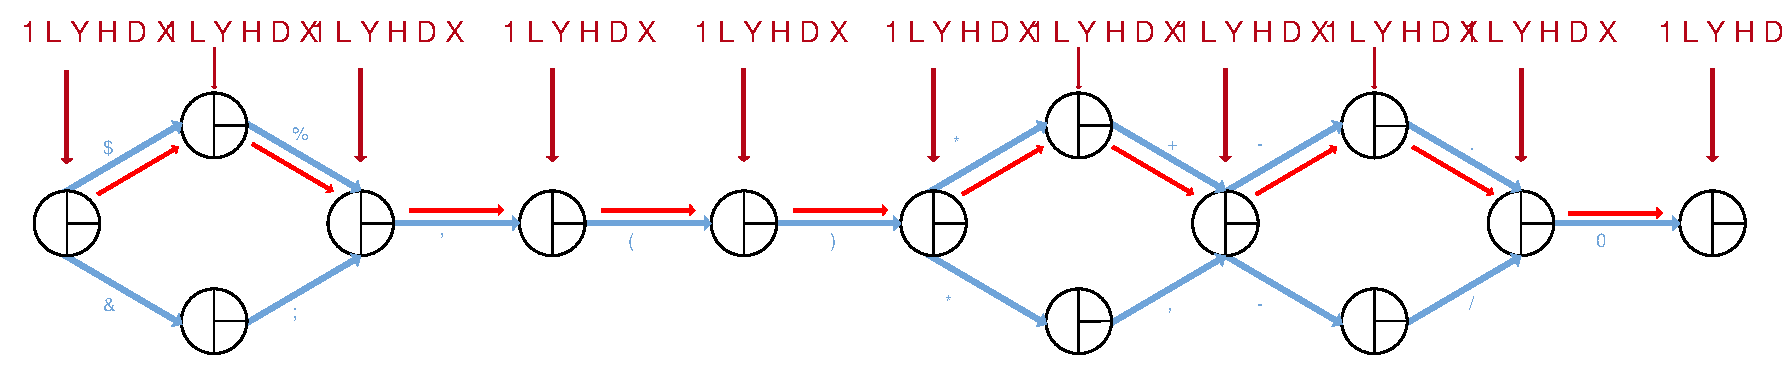
\includegraphics[scale=0.49]
  {textures/images/diagrammes/DiagrammeDePert1.pdf}
  \caption{Diagramme de PERT initial}
  \label{fig:pert-initial}
\end{figure}

Après que le projet soit terminé, j'ai refait le diagramme de PERT afin de coller au plus près au temps passé sur les différentes tâches :

\begin{figure}[h]
  \centering
  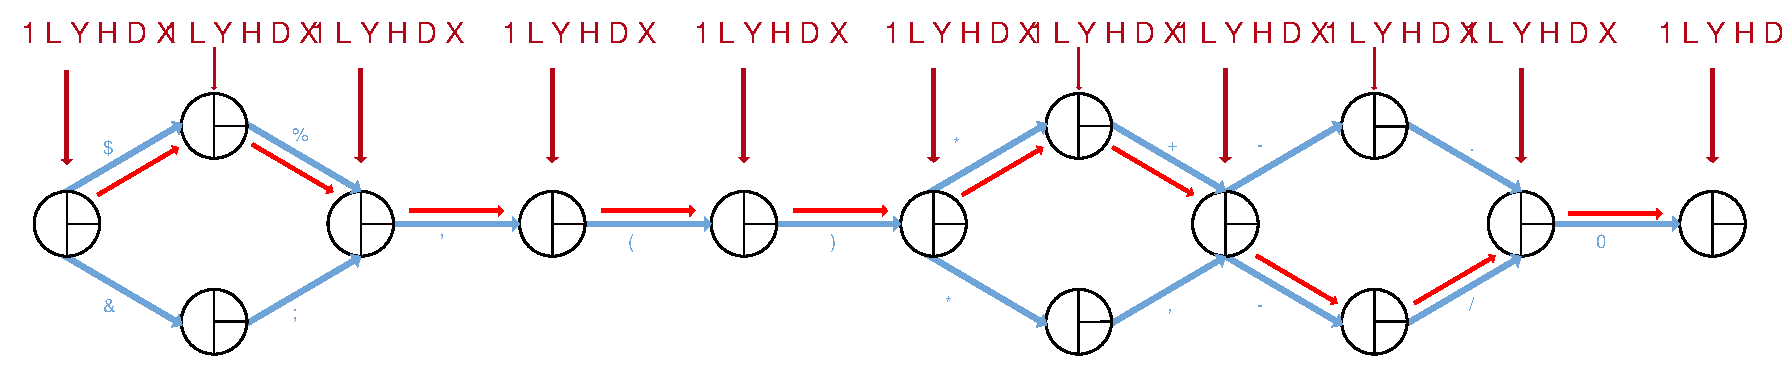
\includegraphics[scale=0.49]
  {textures/images/diagrammes/DiagrammeDePert2.pdf}
  \caption{Diagramme de PERT final}
  \label{fig:pert-final}
\end{figure}

La première chose que l'on peut remarquer, c'est qu'il a fallu moins de temps que prévu pour terminer le projet \textit{(on passe de \textbf{29h15} à \textbf{27h})}. \\

Dans ce diagramme, les tâches sont plus nombreuses pour plus de précision, et leur durée est plus juste. On parle désormais en heures et plus en jours. \\
Par exemple, on peut voir que l'écriture des chapitres dure 8 heures et que celle des exercices en dépend. \\
De même pour la création de la maquette qui ne dépend plus entièrement des tâches ci-dessus. C'est la tâche \textbf{D}, le test de la maquette avec le texte, qui dépend de l'existence du cours, et elle ne dure qu'un quart d'heure.

\newpage

Voici le tableau des antériorités lié au diagramme final :

\begin{figure}[h]
  \centering
  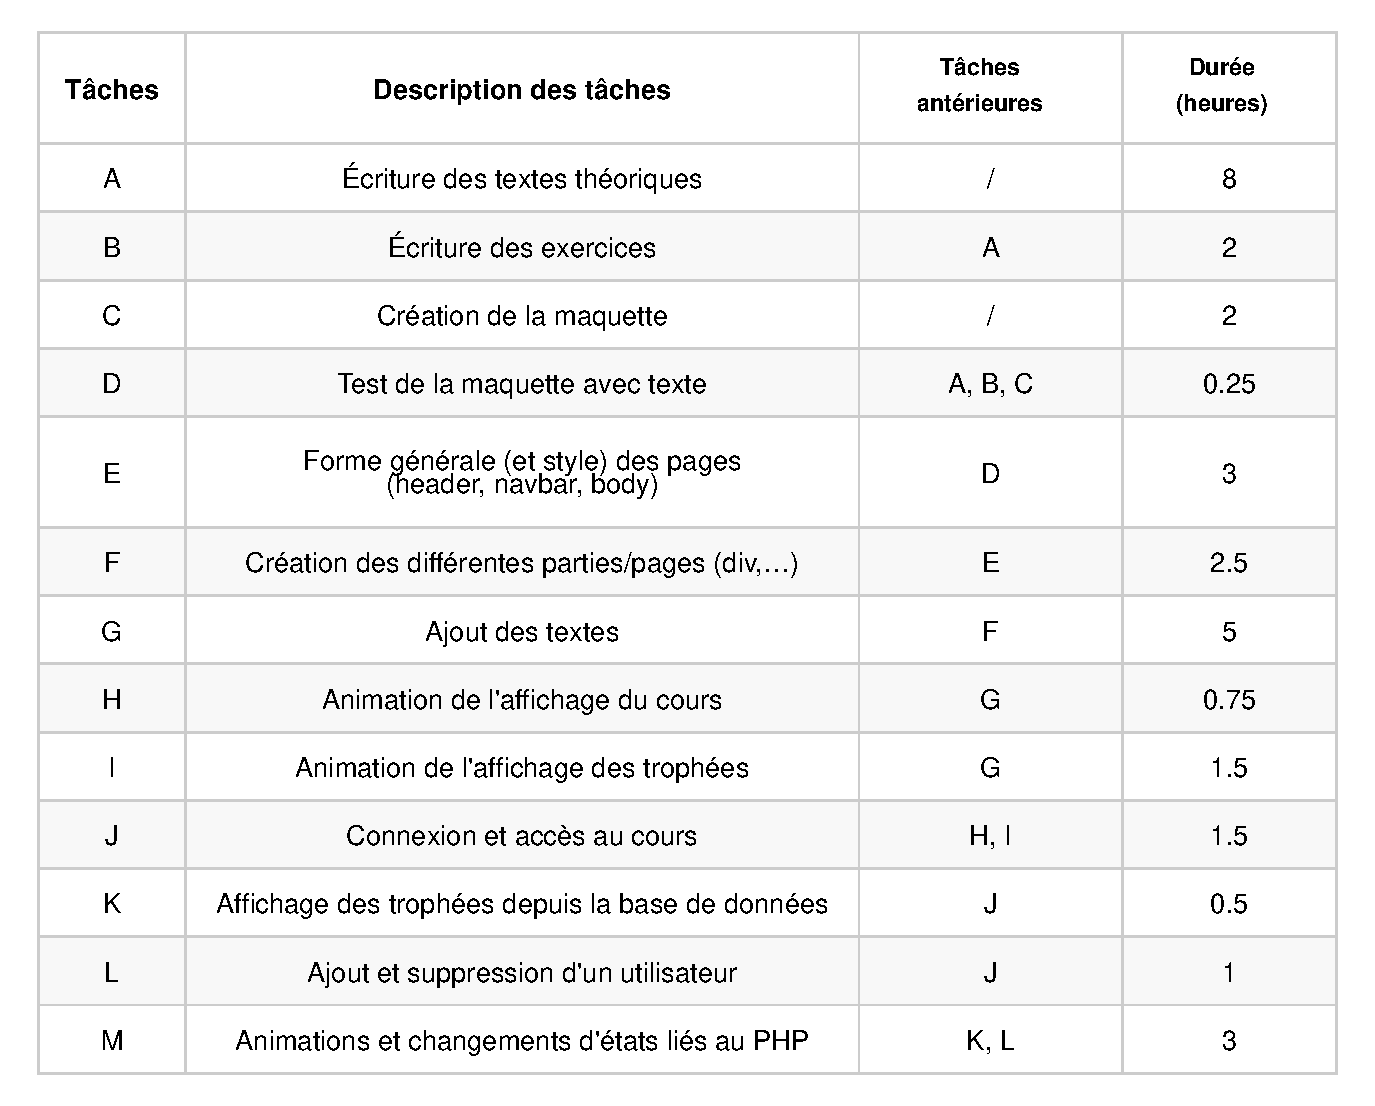
\includegraphics[scale=0.6]
  {textures/images/diagrammes/TableauDesAnteriorites.pdf}
  \caption{Tableau des antériorités}
  \label{fig:tableau-anteriorites}
\end{figure}


{\Large \textbf{Différences entre l'initial et le final}}

Jusqu'à la tâche \textbf{F}, \textit{niveau 7}, il n'y a pas de différences. \\
Après celle-ci, quatre des sept tâches ont eu des durées différentes de ce que j'avais escompté :

\begin{enumerate}

    \item la tâche \textbf{G} est passée de \textbf{1h30} à \textbf{5h}. La cause est simple, la mise en page des chapitres a été plus complexe que prévu.
    En cause, l'ajout de coloration syntaxique, l'ajout de styles pour les types \textit{(gras, italique, etc.)}, ainsi que l'ajout d'un slider \footnote{\url{http://callmenick.com/post/responsive-content-slider}} divisant les chapitres en différentes parties, etc.
    
    \item la connexion à la base de données, tâche \textbf{J}, a pris moins de temps que prévu. \\
    \textbf{Remarquons}, tout de même, que de nombreux changements à ce niveau ont été effectués à la tâche \textbf{M}, dont la raison d'être était de résoudre les problèmes potentiels.
    
    \item l'affichage du résultat dans les trophées \textit{depuis la base de données}, \textit{la tâche \textbf{K}}, a été beaucoup moins difficile qu'imaginé grâce à l'avancée du projet du cours de \textit{Programmation web}.
    
    \item il en est de même pour la tâche \textbf{L}, \textit{l'ajout et la suppression d'utilisateurs}, a donc pris moins de temps.

\end{enumerate}

%%% Local Variables:
%%% mode: latex
%%% TeX-master: t
%%% End:
